\documentclass[12pt]{article}
\usepackage{braket}
\usepackage{physics}
\usepackage{graphicx}
\usepackage{times}
\usepackage[export]{adjustbox}
\usepackage{listings}
\usepackage{mathcomp}
\usepackage{hyperref}
\usepackage{bm,amsmath}
\usepackage{amssymb}
\usepackage{float}
\usepackage{indentfirst}
\usepackage{bigints}
\usepackage{listings}
\usepackage{color}
\usepackage{cite}
\usepackage{slashed}
\hypersetup{
colorlinks=true,
linkcolor=blue,
filecolor=magenta,
urlcolor=cyan,
pdftitle={Overleaf Example},
pdfpagemode=FullScreen,
}
\definecolor{dkgreen}{rgb}{0,0.6,0}
\definecolor{gray}{rgb}{0.5,0.5,0.5}
\definecolor{mauve}{rgb}{0.58,0,0.82}
\lstset{frame=tb,
language=Python,
aboveskip=3mm,
belowskip=3mm,
stepnumber = 1,
showstringspaces=false,
columns=flexible,
basicstyle={\small\ttfamily},
numbers=left,
numberstyle=\color{gray},
keywordstyle=\color{blue},
commentstyle=\color{dkgreen},
stringstyle=\color{mauve},
breaklines=true,
breakatwhitespace=true,
tabsize=3
}
\numberwithin{equation}{section}
\makeindex

\newcommand\be{\begin{eqnarray}}
\newcommand\ee{\end{eqnarray}}
\newcommand\f\phi
\newcommand\cO{\mathcal{O}}
\newcommand\p[1]{\left(#1\right)}
\newcommand\ptl\partial
\newcommand\e\epsilon
\newcommand\<\langle
\renewcommand\>\rangle
\newcommand\Z{\mathbb{Z}}
\newcommand\de\delta
\newcommand\R{\mathbb{R}}
\newcommand\bx{\mathbf{x}}
\newcommand\nn{\nonumber}
\renewcommand\.{\cdot}
\newcommand\x\times
\newcommand\pdr[2]{\frac{\partial #1}{\partial #2}}
\newcommand\s\sigma
\newcommand\SO{\mathrm{SO}}
\newcommand\De{\Delta}
\newcommand\cS{\mathcal{S}}
\newcommand\oo\infty
\newcommand\SU{\mathrm{SU}}
\newcommand\cH{\mathcal{H}}
\newcommand\bn{\mathbf{n}}
\newcommand\bP{\mathbf{P}}
\renewcommand\b\beta
\renewcommand\a\alpha
% \newcommand\Tr{\mathrm{Tr}}
\renewcommand\l\lambda
\newcommand\cL{\mathcal{L}}
\newcommand\cD{\mathcal{D}}
\renewcommand\th{\theta}
\newcommand\tl[1]{\widetilde{#1}}

\title{QFTII Final Project\\Conformal Bootstrap}
\author{Ting-kai Hsu}
\date{\today}

\begin{document}
\maketitle
\tableofcontents
\begin{abstract}
    
\end{abstract}
\section{Introduction}
\section{Quantization and Topological Surface Operator}
\section{Conformal Algebra}
\section{Primary Operator}
\section{Operator Product Expansion}
Consider two operators insertion $\cO_i(x)\cO_j(0)$ inside a spacetime ball $B$ and the path integral over the interior of $B$ gives a state defined on the boundary $\partial B$.  Because every state on the boundary $\partial B$ can be written as a linear combination of primaries and descendants, the state can be decomposed as
\be
\label{eq:opeinitial}
\cO_i(x)\cO_j(0)|0\> &=& \sum_{k}C_{ijk}(x,P)\cO_k(0) |0\>,
\ee
where $k$ runs over primary operators and $C_{ijk}(x,P)$ is an operator that packages together primaries and descendants in the $k$-th conformal multiplet (figure~\ref{fig:ope}), which becomes a coefficient depending on primary operators as the position is taken to be closed to origin $x\rightarrow 0$.

\begin{figure}[H]
\begin{center}
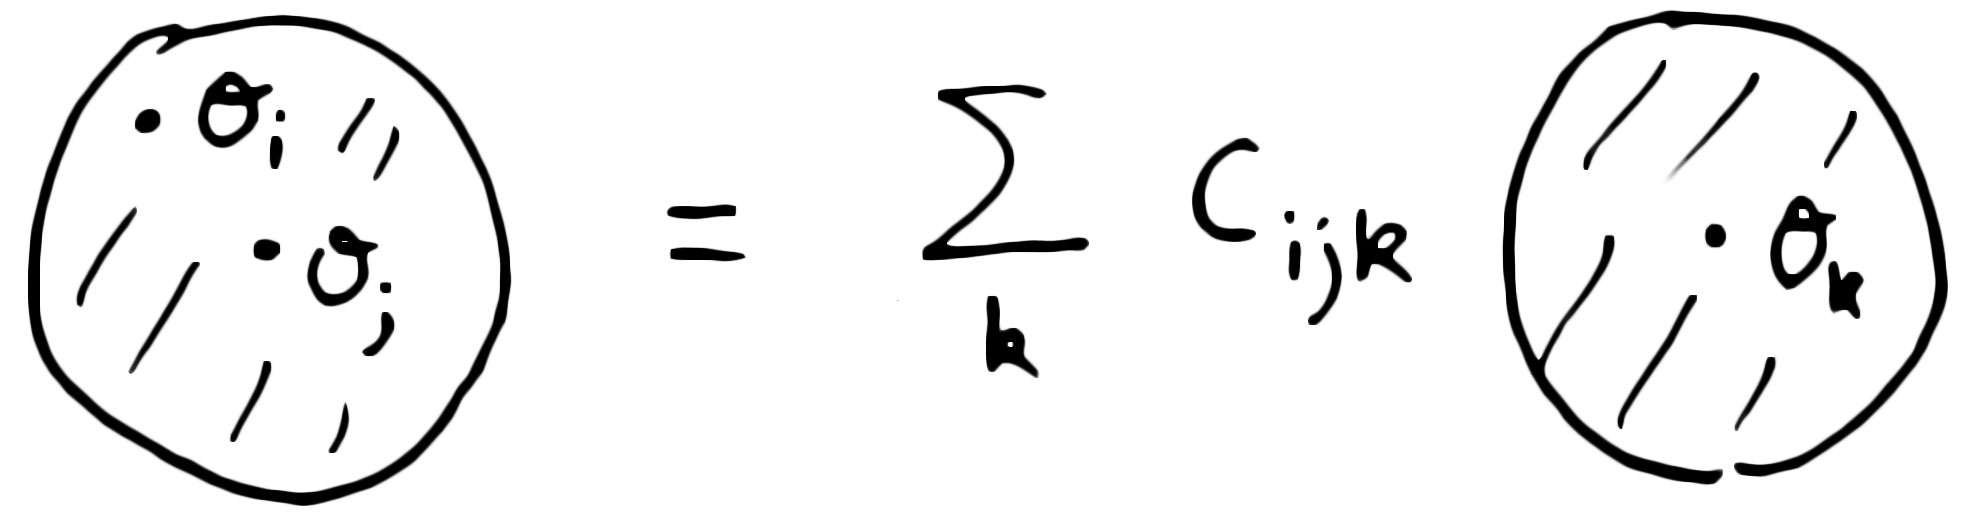
\includegraphics[width=0.6\textwidth]{ope.jpg}
\end{center}
\caption{A state created by two operator insertions can be expanded as a sum of primary states with position-dependent coefficient.  
\label{fig:ope}}
\end{figure}

Using the state-operator correspondence and promoting the momentum operator $P\rightarrow\partial$
\be
\label{eq:opeinitial2}
\cO_i(x_1)\cO_j(x_2) &=& \sum_{k}C_{ijk}(x_{12},\ptl_2)\cO_k(x_2),\qquad\textrm{(OPE)}
\ee
where it is understood that (\ref{eq:opeinitial2}) is valid inside any correlation function where the other operator insertion $\cO_n(x_n)$ far away from them, $|x_{2n}|\geq |x_{12}|$.  Eq.~(\ref{eq:opeinitial2}) is called the Operator Product Expansion (OPE). Operator product expansion can be thought as an analog to Taylor expansion in calculus, and extract the divergence of infinite fluctuation due to small separation into coefficients, with the remaining part represented by a single operator.

We could alternatively perform radial quantization around a different point $x_3$, giving
\be
\label{eq:opealternative}
\cO_i(x_1)\cO_j(x_2) &=& \sum_k C'_{ijk}(x_{13},x_{23},\ptl_3)\cO_k(x_3),
\ee
where $C'_{ijk}(x_{13},x_{23},\ptl_3)$ is some other differential operator (figure~\ref{fig:radialquantotherpoint}).  The form  (\ref{eq:opeinitial2}) is usually more convenient for computations, but the existence of (\ref{eq:opealternative}) is important. It shows that we can do the OPE between two operators whenever it's possible to draw any sphere that separates the two operators from all the other operator insertion in path integral.

\begin{figure}[h]
\begin{center}
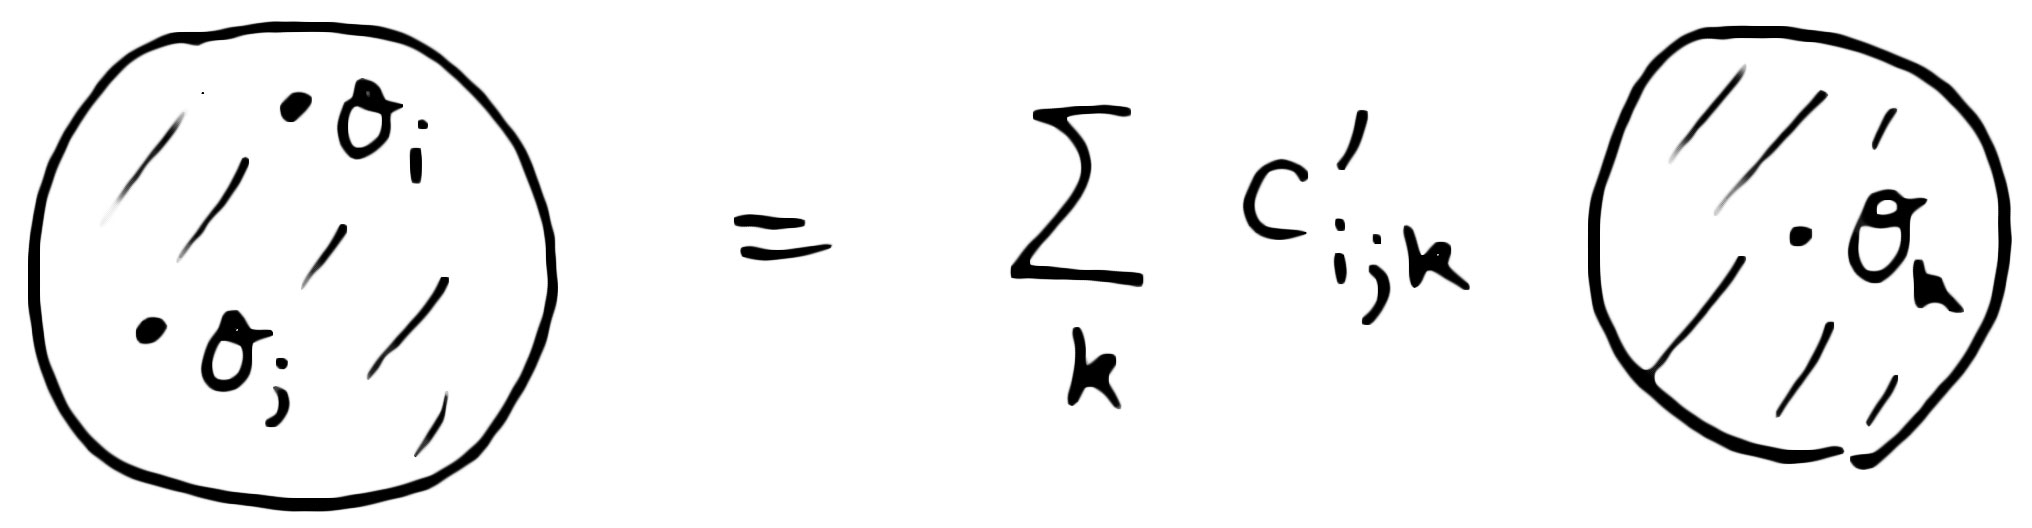
\includegraphics[width=0.6\textwidth]{radialquantotherpoint.jpg}
\end{center}
\caption{OPE doesn't have to centered at origin, and the expansion basis is located at some spacetime point as the  dependence 
 of the other operator's position is absorbed by the coefficients. \label{fig:radialquantotherpoint}}
\end{figure}

It's possible for all the operators to have spin indices.  In this case, the OPE then becomes
\be
\cO_i^a(x_1)\cO_j^b(x_2) &=& \sum_k C_{ijk}^{ab}{}_c(x_{12},\ptl_2)\cO_k^c(x_2),
\ee
where $a,b,c$ are indices for (possibly different) representations of $\SO(d)$.

By acting on both sides of (\ref{eq:opeinitial}) with $D$, one can prove that $C_{ijk}(x,\ptl)$ has an expansion of the form
\be
\label{eq:opeexpansionexample}
C_{ijk}(x,\ptl) &\propto& |x|^{\De_k-\De_i-\De_j}\p{1 +\# x^\mu\ptl_\mu + \# x^\mu x^\nu\ptl_\mu\ptl_\nu+\# x^2 \ptl^2 + \dots}\nn\\
\ee
\subsection{Consistency with Conformal Invariance}
% \begin{exercise}
% \end{exercise}
By conformal invariance, such as dimensional analysis, rotational invariance, and non-trivially, the special conformal transform $K_{\mu}$, the form of the coefficient in OPE is strongly restricted.

We get a more interesting constraint by acting with $K_\mu$, for simplicity, suppose $\cO_i$, $\cO_j$, and $\cO_k$ are scalars. In fact, consistency with $K_\mu$ completely fixes $C_{ijk}$ up to an overall coefficient. In this way, we can determine the coefficients in (\ref{eq:opeexpansionexample}).

Why the form of the OPE is fixed? To get the coefficients in (\ref{eq:opeexpansionexample}), take the correlation function of both sides of (\ref{eq:opeinitial2}) with a third operator $\cO_k(x_3)$ (we will assume $|x_{23}|\geq |x_{12}|$, so that the OPE of $O_i\text{ and }O_j$ is valid),
\be
\label{eq:threetotwo}
\<\cO_i(x_1)\cO_j(x_2)\cO_k(x_3)\> &=& \sum_{k'} C_{ijk'}(x_{12},\ptl_2)\<\cO_{k'}(x_2)\cO_k(x_3)\>.
\ee

The three-point function on the left-hand side is fixed by conformal invariance, as mentioned in the previous sections. Choosing \textbf{an orthonormal basis of primary operators} for the expansion, so that $\<\cO_k(x_2)\cO_{k'}(x_3)\>= \de_{kk'}x_{23}^{-2\De_k}$.  The sum then collapses to a single term, giving
\be
\label{eq:matchingthreept}
\frac{f_{ijk}}{x_{12}^{\De_i+\De_j-\De_k}x_{23}^{\De_j+\De_k-\De_i}x_{31}^{\De_k+\De_i-\De_j}} &=& C_{ijk}(x_{12},\ptl_2)x_{23}^{-2\De_k}.
\ee
This determines $C_{ijk}$ to be proportional to $f_{ijk}$, times a differential operator that depends only on the $\De_i$'s. The coefficient operator can be obtained by matching both sides of (\ref{eq:matchingthreept}) in small expansion $|x_{12}|/|x_{23}|$.
% \begin{exercise}
% \label{exercise:seriesfordiffops}

Consider the special case $\De_i=\De_j=\De_\f$, and $\De_k=\De$.  Show
\be
\label{eq:identicalscalaropeoperator}
C_{ijk}(x,\ptl) &=& f_{ijk} x^{\De-2\De_\f}\p{1+\frac 1 2 x\.\ptl + \a x^\mu x^\nu\ptl_\mu\ptl_\nu + \b x^2 \ptl^2+\dots},\nn\\
\ee
where
\be
\label{eq:opedescendantcoefficients}
\a &=& \frac{\De+2}{8(\De+1)},\quad\textrm{and}\quad \b=-\frac{\De}{16(\De-\frac{d-2}{2})(\De+1)}.
\ee
% \end{exercise}

\subsection{Correlation Function with OPE}

Equation (\ref{eq:threetotwo}) gives an example of using the OPE to reduce a three-point function to a sum of two-point functions.  In general, we can use the OPE to reduce any $n$-point function to a sum of $n-1$-point functions by assumption of locality,
\be
\<\cO_1(x_1)\cO_2(x_2)\cdots\cO_n(x_n)\> &=& \sum_k C_{12k}(x_{12},\ptl_2)\<\cO_k(x_2)\cdots\cO_n(x_n)\>.\nn\\
\ee
Recursing, we can reduce everything to a sum of one-point functions, which are fixed by dimensional analysis,
\be
\<\cO(x)\> &=& \begin{cases}
1 & \textrm{if $\cO$ is the unit operator,}\\
0 & \textrm{otherwise.}
\end{cases}
\ee
This gives an algorithm for computing any flat-space correlation function using the OPE\@.  It shows that all these correlation functions are determined by dimensions $\De_i$, spins, and three-point correlation function coefficients $f_{ijk}$.
% \footnote{The OPE is also valid on any conformally flat manifold.  The difference is that on nontrivial manifolds, non-unit operators can have nonzero one-point functions.  An example is $\R^{d-1}\x S^1_\b$, which has the interpretation as a CFT at finite temperature.  By dimensional analysis, we have $\<\cO\>_{\R^{d-1}\x S^1_\b}\propto \b^{-\De_\cO}\propto T^{\De_\cO}$.\label{foot:finitetemperature}}

\section{Conformal Blocks}

\subsection{Using the OPE}

We can use the OPE to compute a four-point correlation function of identical scalars. Recall that conformal invariance fixes the function up to some arbitrary function that is conformal-invariant
\be
\<\f(x_1)\f(x_2)\f(x_3)\f(x_4)\> &=& \frac{g(u, v)}{x_{12}^{\De_\f}x_{34}^{\De_\f}},
\ee
where the cross-ratios $u$, $v$ are given previous section.

On the other hand, the OPE of two scalar field takes the form
\be
\label{eq:scalarscalarOPE}
\f(x_1)\f(x_2) &=& \sum_\cO f_{\f\f\cO} C_{a}(x_{12},\ptl_2)\cO^{a}(x_2),
\ee
where $\cO^{a}$ can have nonzero spin in general. 
% For $\cO^a$ to appear in the OPE of two scalars, it must transform in a spin-$\ell$ traceless symmetric tensor representation of $\SO(d)$.
% \begin{exercise}

% Prove this as follows. Show that $\<\cO^a|\f(x)|\f\>$ vanishes unless $\cO^a$ is a symmetric tensor.  (Tracelessness comes from restricting to irreducible representations of $\SO(d)$.) Argue that if $\<\cO^a|\f(x)|\f\>$ vanishes, then for any descendant $|\psi\>=P\cdots P|\cO\>$, the matrix element $\<\psi|\f(x)|\f\>$ vanishes as well.
% \end{exercise}
% \begin{exercise}

\noindent\rule[0.5ex]{\linewidth}{1pt}
\label{exercise:elleven}
Using the three-point correlation function, show that $f_{\f\f\cO}$ vanishes unless $\ell$ is even.
% \end{exercise}

\noindent\rule[0.5ex]{\linewidth}{1pt}

We can pair up the operator (12)(34) by assuming their relative positions are separated well to avoid operator insertions crossing, and then we can do the OPE in pairs,\footnote{Although this computation will look like we need $x_{3,4}$ to be sufficiently far from $x_{1,2}$, it in fact will be correct whenever we can draw any sphere separating $x_1,x_2$ from $x_3,x_4$, and this is because the beautiful scale invariance in CFT.}
\begin{align}
\label{eq:fourptcalc}
\<
\contraction{}{\f}{(x_1)}{\f}
\f(x_1)&\f(x_2)
\contraction{}{\f}{(x_1)}{\f}
\f(x_3)\f(x_4)
\>\nn\\
&= \sum_{\cO,\cO'}f_{\f\f\cO}f_{\f\f\cO'} C_a(x_{12},\ptl_2)C_b(x_{34},\ptl_4)\<\cO^a(x_2)\cO'^b(x_4)\>\nn\\
&= \sum_\cO f_{\f\f\cO}^2 C_a(x_{12},\ptl_2)C_b(x_{34},\ptl_4)\frac{I^{ab}(x_{24})}{x_{24}^{2\De_\cO}}\nn\\
&= \frac{1}{x_{12}^{\De_\f} x_{34}^{\De_\f}}\sum_\cO f_{\f\f\cO}^2 g_{\De_\cO,\ell_\cO}(x_i),
\end{align}

where
\be
\label{eq:olddefinitionofg}
g_{\De,\ell}(x_i) &\equiv& x_{12}^{\De_\f} x_{34}^{\De_\f} C_a(x_{12},\ptl_2)C_b(x_{34},\ptl_4)\frac{I^{ab}(x_{24})}{x_{24}^{2\De}}.
\ee
In (\ref{eq:fourptcalc}), we have chosen an orthonormal basis of operators and used that
\be
\label{eq:canonicallynormalizedtwopt}
\<\cO^a(x)\cO'^b(0)\> &=& \de_{\cO\cO'} \frac{I^{ab}(x)}{x^{2\De_\cO}},
\ee
where $I^{ab}(x)=I^{\mu_1\cdots\mu_\ell,\nu_1\cdots\nu_\ell}(x)$ is the tensor in (\ref{eq:twopointfunctionofspinL}).

The functions $g_{\De,\ell}(x_i)$ are called {\it conformal blocks}.  Although it's not obvious from the way we defined them, it turns out they are actually functions of the conformal cross-ratios $u,v$ alone.  We thus have the conformal block decomposition
\be
g(u,v) &=& \sum_\cO f_{\f\f\cO}^2 g_{\De_\cO,\ell_\cO}(u,v).
\ee
% \begin{exercise}
Using the differential operator (\ref{eq:identicalscalaropeoperator}), show
\be
\label{eq:boundaryconditionforblock}
g_{\De,0}(u,v) &=& u^{\De/2}\p{1+\dots}.
\ee
% \end{exercise}

% \begin{exercise}
Using (\ref{eq:scalarscalarspinL}), argue that $x^{2\De_\f} C_{\f\f\cO}(x,\ptl)$ is independent of $\Delta_\phi$ for any spin of $\cO$. Conclude that $g_{\De,\ell}(u,v)$ is independent of $\Delta_\phi$. (This is a special property of conformal blocks for operators with identical scaling dimensions.)
% \end{exercise}


\subsection{In Radial Quantization}

A conformal block represents the contribution of a single conformal multiplet to a four-point function.  It is instructive to understand it in radial quantization.  Along the way, we'll explain why the blocks are functions of the cross-ratios $u,v$ alone.

Let us pick an origin such that $|x_{3,4}|\geq |x_{1,2}|$, so that
\be
\label{eq:fourptradial}
\<\f(x_1)\f(x_2)\f(x_3)\f(x_4)\> &=& \<0|\mathcal{R}\{\f(x_3)\f(x_4)\}\mathcal{R}\{\f(x_1)\f(x_2)\}|0\>.\quad
\ee
For a primary operator $\cO$, let $|\cO|$ be the projector onto the conformal multiplet of $\cO$,
\be
|\cO| &\equiv& \sum_{\a,\b=\cO,P\cO,PP\cO,\dots} |\a\>\mathcal{N}^{-1}_{\a\b}\<\b|,\qquad
\mathcal{N}_{\a\b} \equiv \<\a|\b\>.
\ee
The identity is the sum of these projectors over all primary operators.
\be
\mathbf{1} &=& \sum_\cO |\cO|.
\ee
Inserting this into (\ref{eq:fourptradial}) gives
\be
\label{eq:insertingprojector}
\<\f(x_1)\f(x_2)\f(x_3)\f(x_4)\> &=& \sum_\cO\<0|\mathcal{R}\{\f(x_3)\f(x_4)\}|\cO|\mathcal{R}\{\f(x_1)\f(x_2)\}|0\>.\nn\\
\ee
Each term in the sum is a conformal block times a squared OPE coefficient and some conventional powers of $x_{ij}$,
\be
\label{eq:newdefinitionofg}
\<0|\mathcal{R}\{\f(x_3)\f(x_4)\}|\cO|\mathcal{R}\{\f(x_1)\f(x_2)\}|0\> &=& \frac{f_{\f\f\cO}^2}{x_{12}^{2\De_\f}x_{34}^{2\De_\f}}g_{\De_\cO,\ell_\cO}(u,v).\qquad
\ee
% \begin{exercise}

Verify the equivalence between (\ref{eq:newdefinitionofg}) and (\ref{eq:olddefinitionofg}) by performing the OPE between $\f(x_3)\f(x_4)$ and $\f(x_1)\f(x_2)$.
% \end{exercise}


This expression makes it clear why $g_{\De,\ell}(u,v)$ is a function of $u$ and $v$: the projector $|\cO|$ commutes with all conformal generators (by construction).  Thus, the object above satisfies all the same Ward identities as a four-point function of primaries, and it must take the form (\ref{eq:fourptfunctionofprimaries}).  In path integral language, we can think of $|\cO|$ as a new type of  surface operator.  Here, we've inserted it on a sphere separating $x_{1,2}$ from $x_{3,4}$.

\subsection{From the Conformal Casimir}

We can now give a simple and elegant way to compute the conformal block, due to Dolan \& Osborn \cite{DO2}.
Recall that the conformal algebra is isomorphic to $\SO(d+1,1)$, with generators $L_{ab}$ given by (\ref{eq:conformalgeneratorssodplus11}).  The Casimir $C=-\frac 1 2 L^{ab}L_{ab}$ acts with the same eigenvalue on every state in an irreducible representation.  
% \begin{exercise}

Show that this eigenvalue is given by
\be
C|\cO\> &=& \l_{\De,\ell}|\cO\>,\nn\\
\l_{\De,\ell} &\equiv& \De(\De-d)+\ell(\ell+d-2).
\ee
% \end{exercise}

It follows that $C$ gives this same eigenvalue when acting on the projection operator $|\cO|$ from either the left or right,
\be
C|\cO|=|\cO| C = \l_{\De,\ell}|\cO|.
\ee

Let $\cL_{ab,i}$ be the differential operator giving the action of $L_{ab}$ on the operator $\f(x_i)$.  Note that
\be
(\cL_{ab,1}+\cL_{ab,2})\f(x_1)\f(x_2)|0\> &=& \p{[L_{ab},\f(x_1)]\f(x_2)+\f(x_1)[L_{ab},\f(x_2)]}|0\>\nn\\
&=& L_{ab}\f(x_1)\f(x_2)|0\>.
\ee
Thus, 
\be
C\f(x_1)\f(x_2)|0\> &=& \cD_{1,2}\f(x_1)\f(x_2)|0\>,\nn\\
\textrm{where}\qquad\cD_{1,2} &\equiv& -\frac 1 2(\cL^{ab}_{1}+\cL^{ab}_{2})(\cL_{ab,1}+\cL_{ab,2}).
\ee
We then have
\begin{align}
\cD_{1,2}\<0|&\mathcal{R}\{\f(x_3)\f(x_4)\}|\cO|\mathcal{R}\{\f(x_1)\f(x_2)\}|0\>\nn\\
&=
\<0|\mathcal{R}\{\f(x_3)\f(x_4)\}|\cO| C\mathcal{R}\{\f(x_1)\f(x_2)\}|0\>\nn\\
&= \l_{\De,\ell}\<0|\mathcal{R}\{\f(x_3)\f(x_4)\}|\cO|\mathcal{R}\{\f(x_1)\f(x_2)\}|0\>.
\end{align}
Plugging in (\ref{eq:newdefinitionofg}), we find that $g_{\De,\ell}$ satisfies the differential equation 
\be
\label{eq:conformalcasimir}
\cD g_{\De,\ell}(u,v) &=& \l_{\De,\ell} g_{\De,\ell}(u,v),
\ee
where the second-order differential operator $\cD$ is given by
\be
\cD &=& 2(z^2(1-z)\ptl_z^2-z^2 \ptl_z) + 2(\bar z^2 (1-\bar z)\ptl_{\bar z}^2-\bar z^2 \ptl_{\bar z})\nn\\
&& + 2(d-2)\frac{z\bar z}{z-\bar z}((1-z)\ptl_z - (1-\bar z)\ptl_{\bar z}).
\ee

Eq.~(\ref{eq:conformalcasimir}), together with the boundary condition~(\ref{eq:boundaryconditionforblock}) (and its generalization to nonzero spin, which we give shortly), then determines the conformal block $g_{\Delta,\ell}(u,v)$.  In even dimensions, the Casimir equation can be solved analytically.  For example, in 2d and 4d \cite{DO1,DO2},
\be
\label{eq:explicitblock2d}
g_{\De,\ell}^{(2d)}(u,v) &=& k_{\De+\ell}(z)k_{\De-\ell}(\bar z) + k_{\De-\ell}(z)k_{\De+\ell}(\bar z),\\
\label{eq:explicitblock4d}
g_{\De,\ell}^{(4d)}(u,v) &=& \frac{z \bar z}{z-\bar z}\p{k_{\De+\ell}(z)k_{\De-\ell-2}(\bar z) - k_{\De-\ell-2}(z)k_{\De+\ell}(\bar z)},\\
k_\beta(x) &\equiv& x^{\beta/2}{}_2F_1\p{\frac \beta 2, \frac \beta 2, \beta, x}.
\ee
In odd dimensions, no explicit formula in terms of elementary functions is known.  However the blocks can still be computed in a series expansion using the Casimir equation or alternative techniques like recursion relations.

\subsection{Series Expansion}

It will be helpful to understand the series expansion of the conformal blocks in more detail.
 The ``radial coordinates" of \cite{Pappadopulo:2012jk,Hogervorst:2013sma} are ideal for this purpose.
 Using conformal transformations, we can place all four operators on a plane in the configuration shown in figure~\ref{fig:rho}.  This makes it clear that the conformal block expansion is valid whenever $|\rho|<1$.

\begin{figure}
\begin{center}
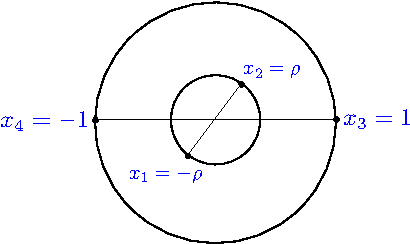
\includegraphics[width=0.55\textwidth]{fig-rho}
\end{center}
\caption{Any four points can be brought to the above configuration using conformal transformations. (Figure from \cite{Hogervorst:2013sma}.)  \label{fig:rho}}
\end{figure}

% \begin{exercise}
Show that $\rho=re^{i\theta}$ is related to $z$ via
\be
\label{eq:radialcoordinatedefinition}
\rho = \frac{z}{(1+\sqrt{1-z})^2},\qquad z = \frac{4\rho}{(1+\rho)^2}
\ee
(and similarly for $\bar\rho=r e^{-i\theta}$ and $\bar z$).
% \end{exercise}

In radial quantization, this corresponds to placing cylinder operators (\ref{eq:definitionofcylinderop}) at diametrically opposite points $\pm \bn$ and $\pm \bn'$ on $S^{d-1}$, with $\cos\th=\bn\.\bn'$, and with the pairs separated by time $\tau=-\log r$ (figure~\ref{fig:cylinderconfig}).  The conformal block is then
\be
\label{eq:blockintermsofpsi}
 g_{\De,\ell}(u,v) &=& \<\psi(\bn)||\cO|e^{-\tau D}|\psi(\bn')\>,
\ee
where we've defined the state\footnote{The factor $2^{\De_\f}=\<\f_\mathrm{cyl.}(0,\bn)\f_\mathrm{cyl.}(0,-\bn)\>^{-1}$ comes from transforming $x_{12}^{-2\De_\f}$ to the cylinder (exercise!).}
\be
|\psi(\bn)\> &\equiv& \frac{2^{\De_\f}}{f_{\f\f\cO}}\phi_\mathrm{cyl.}(0,\bn)\phi_\mathrm{cyl.}(0,-\bn)|0\>.
\ee


\begin{figure}
\begin{center}
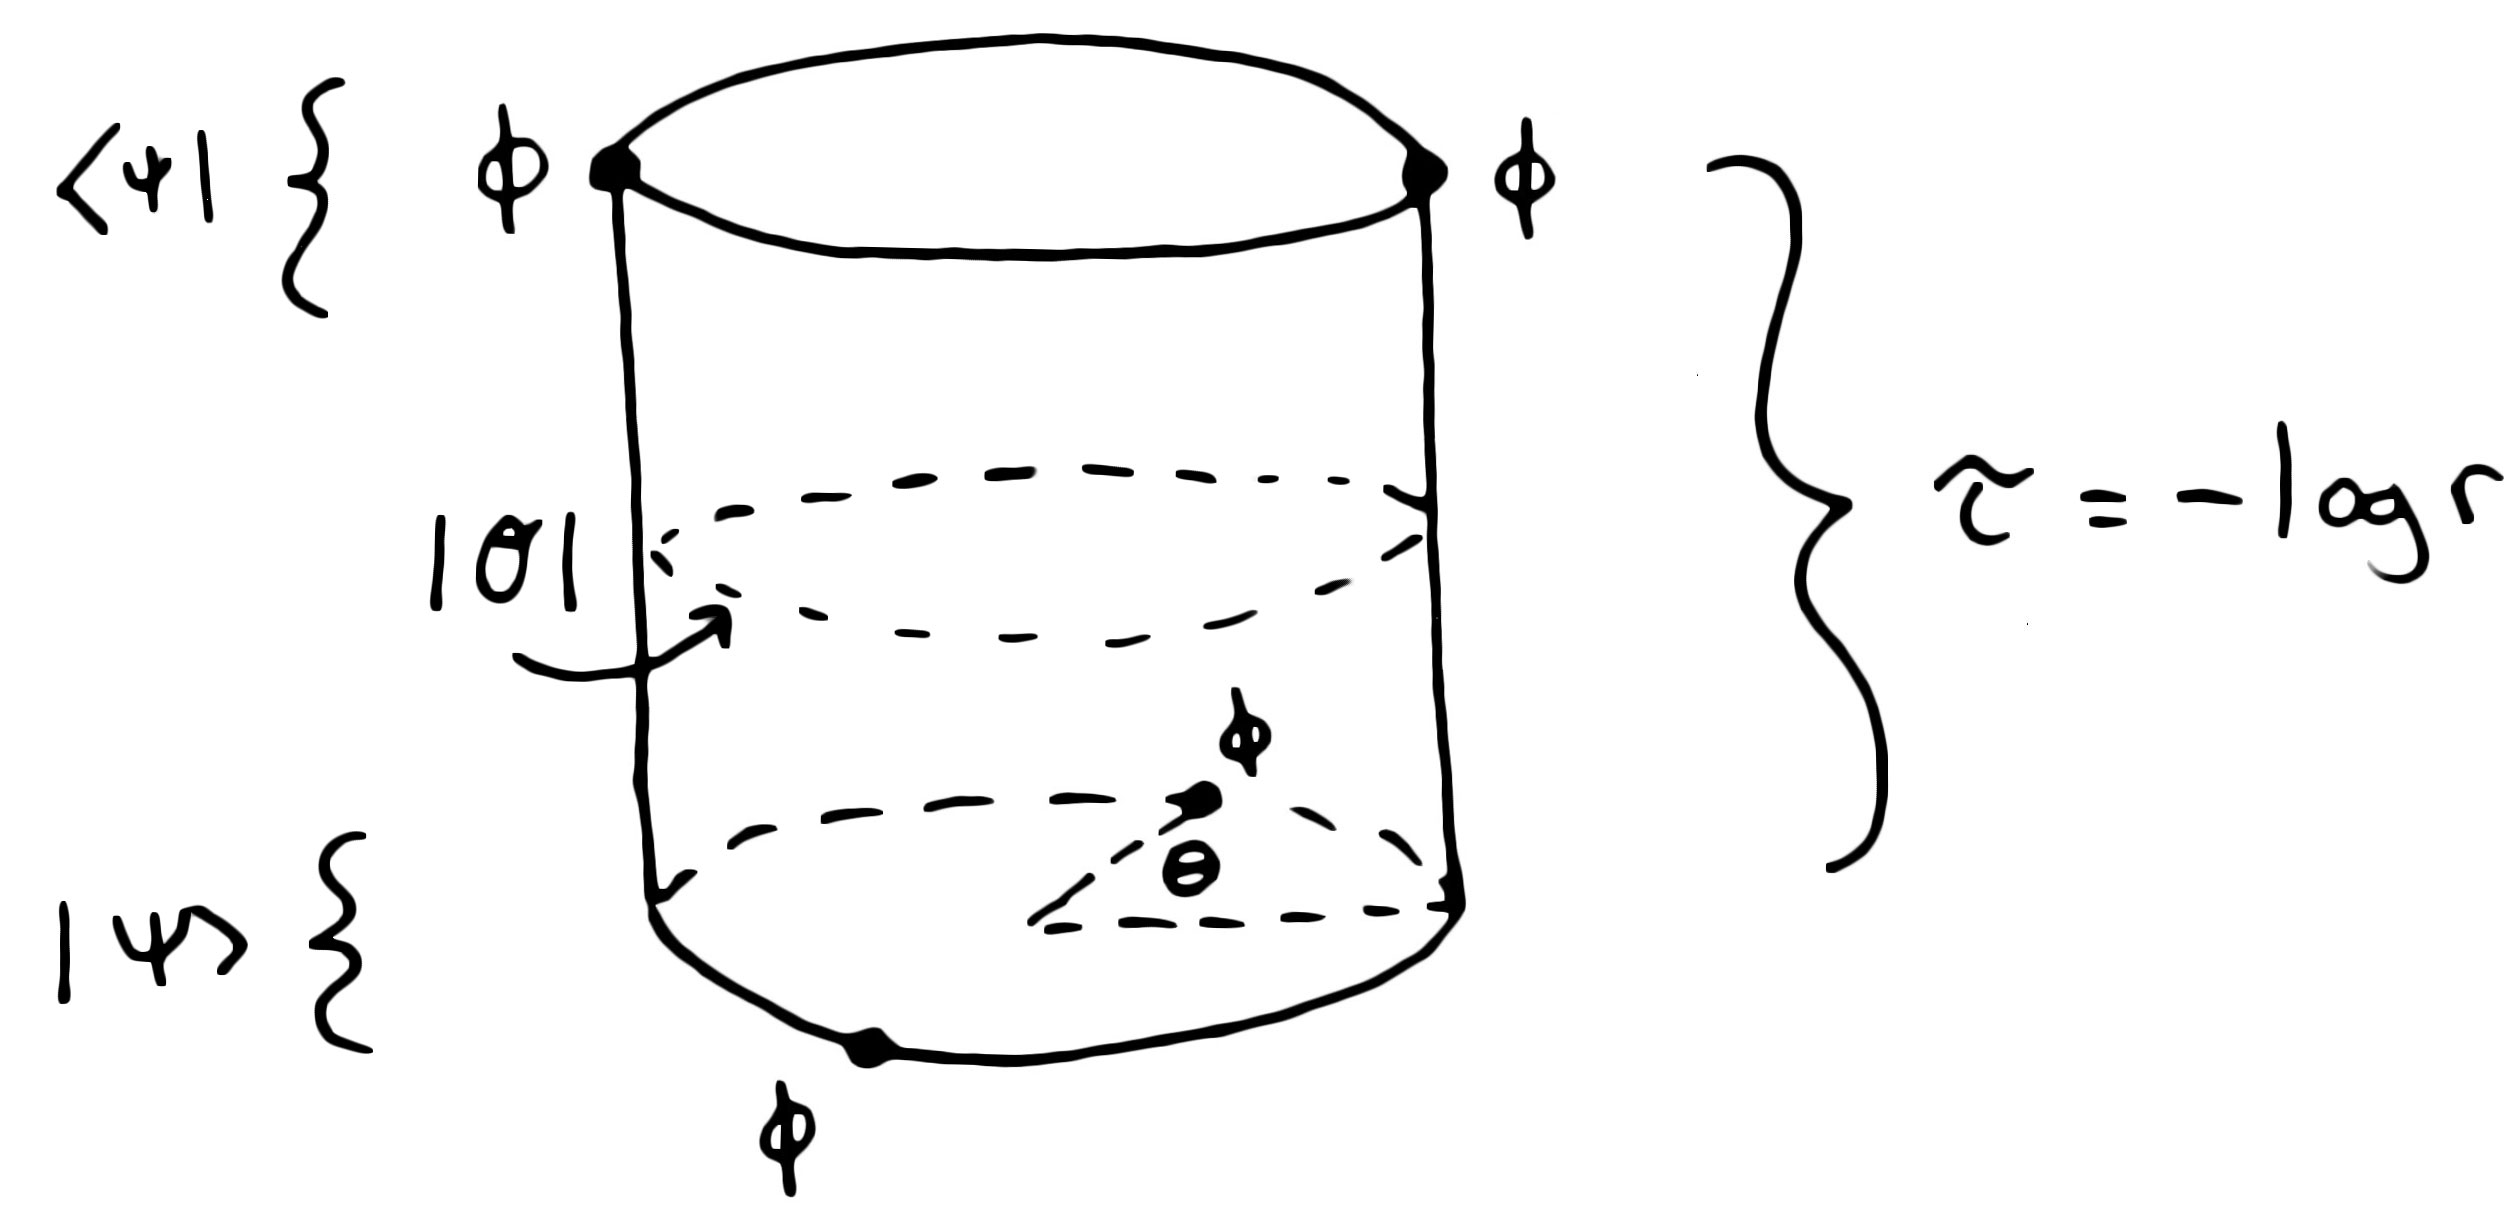
\includegraphics[width=0.75\textwidth]{cylinderconfig.jpg}
\end{center}
\caption{Configuration on the cylinder corresponding to (\ref{eq:blockintermsofpsi}).  \label{fig:cylinderconfig}}
\end{figure}

A descendant $P^{\mu_1}\cdots P^{\mu_n}|\cO\>$ has energy $\De+n$ on the cylinder.  Within the $n$-th energy level, the $\SO(d)$ spins that appear are
\be
\label{eq:rangeofjs}
j \in \{\ell+n,\ell+n-2,\dots,\mathrm{max}(\ell-n,\ell+n\,\,\mathrm{mod}\,\,2)\}.
\ee
Consider a set of descendant states $|n,j\>^{\mu_1\cdots\mu_j}$ with energy $\De+n$ and spin $j$. They contribute
\be
r^{\De+n} \<\psi(\bn)|n,j\>^{\mu_1\cdots\mu_j}{}_{\mu_1\cdots\mu_j}\<n,j|\psi(\bn')\>.
\label{eq:definitespinandenergy}
\ee
By rotational invariance,
\be
\<\psi(\bn)|n,j\>^{\mu_1\cdots\mu_j} &\propto& \bn^{\mu_1}\cdots\bn^{\mu_j}-\mathrm{traces}.
\ee
Because $|\psi(\bn)\>=|\psi(-\bn)\>$, $j$ must be even (and thus $n$ is even).
The contraction of two traceless symmetric tensors is a Gegenbauer polynomial,
\be
C_j^{\frac{d-2}{2}}(\bn\cdot\bn') &\propto& (\bn^{\mu_1}\cdots\bn^{\mu_j}-\mathrm{traces})(\bn'_{\mu_1}\cdots\bn'_{\mu_j}-\mathrm{traces}),
\ee
so (\ref{eq:definitespinandenergy}) becomes
\be
r^{\De+n} \<\psi(\bn)|n,j\>^{\mu_1\cdots\mu_j}{}_{\mu_1\cdots\mu_j}\<n,j|\psi(\bn')\> &\propto& r^{\De+n}C_j^{\frac{d-2}{2}}(\cos\th).
\ee

Summing over descendants, we find
\be
\label{eq:seriesexpansion}
g_{\De,\ell}(u,v) &=& \sum_{\substack{n=0,2,\dots \\ j}} B_{n,j}r^{\De+n}C_j^{\frac{d-2}{2}}(\cos\th),\label{eq:seriesforblock}
\ee
where $j$ ranges over the values in (\ref{eq:rangeofjs}) and $B_{n,j}$ are constants.  
Notice a few properties:
\begin{itemize}
\item The leading term in the $r$-expansion comes from the primary state $|\cO\>$ with $n=0$ and $j=\ell$. This can be used as a boundary condition in the Casimir equation to determine the higher coefficients $B_{n,j}$.
\item The $B_{n,j}$ are positive in a unitary theory because they are given by norms of projections of $|\psi\>$ onto energy and spin eigenstates.
\item The $B_{n,j}$ are rational functions of $\De$.  This follows because the Casimir eigenvalue $\l_{\De,\ell}$ is polynomial in $\De$, or alternatively from the fact that the differential operators $C_a(x,\ptl)$ appearing in the OPE (\ref{eq:scalarscalarOPE}) have a series expansion in $x$ with rational coefficients, see exercise~\ref{exercise:seriesfordiffops}. 
\end{itemize}

% \begin{exercise}
Expand $g^{(2d)}_{\De,\ell}(u,v)$ and $g^{(4d)}_{\De,\ell}(u,v)$ to the first few orders in $r$, and check these properties.  Verify that some of the coefficients $B_{n,j}$ become negative when $\De$ violates the unitarity bound.
% \end{exercise}

% \begin{exercise}
By rewriting in terms of $r,\th$ and using (\ref{eq:seriesexpansion}), show that even spin blocks are invariant under $x_1\leftrightarrow x_2$ or $x_3\leftrightarrow x_4$,
\be
\label{eq:invariantunderonetwo}
g_{\De,\ell}(u,v) &=& g_{\De,\ell}\p{\frac{u}{v},\frac 1 v},\qquad(\textrm{$\ell$ even}).
\ee
% \end{exercise}

\section{2d Ising CFT and Conformal Bootstrap}


\section{Introduction to Conformal Bootstrap and Its Language}

This section encompasses the first three chapters of Simmons-Duffin's TASI lecture notes \cite{simmonsduffin2016tasilecturesconformalbootstrap}, where we provide a brief overview of the bootstrapping philosophy, along with the foundational language and conventions used in this field.

\subsection{Bootstrap Philosophy}
Critical universality of many microscopic theories allows us to focus on the CFT.

\subsection{Path Integral Quantization}
Path integral formalism chooses a specific time direction, and spacetime is divided into successive slices. Each slice is associated with a Hilbert space of states in the Heisenberg picture, and the progression from one slice to the next is governed by time evolution. The general correlator is defined as follows:

\begin{equation}
    \langle\mathcal{O}_1(x_1)\cdots\mathcal{O}_n(x_n)\rangle = \bra{0}\text{T}\left\{\hat{\mathcal{O}_1}(t_1,\mathbf{x}_1)\cdots\hat{\mathcal{O}_n}(t_n,\mathbf{x}_n)\right\}\ket{0}
\end{equation}

Here, note that the L.H.S represents a product of spacetime functions. At the same time, the R.H.S. is a product of operators in the Heisenberg picture, defined in distinct Hilbert spaces corresponding to each slice. This is the familiar form of the correlator within the path integral framework.

\subsection{Stress Energy and Topological Surface Operator}
Consider a quantum field theory (QFT) coupled to a background metric $g$,  with correlators defined within the path integral formalism in Euclidean signature. 
\begin{equation}
    \bra{0}\text{T}\left\{\hat{\mathcal{O}_1}(t_1,\mathbf{x}_1)\cdots\hat{\mathcal{O}_n}(t_n,\mathbf{x}_n)\right\}\ket{0}_{g} = \int{\prod_{y}d\phi(y)\,\mathcal{O}_1(x_1)\cdots\mathcal{O}_n(x_n)e^{-S[g,\phi]}}
\end{equation}
The stress-energy tensor acts as the conserved current associated with the diffeomorphism invariance of the action $S[g,\phi]$ in the flat spacetime limit $g\rightarrow\eta$.
% \begin{equation}
%     \langle T^{\mu\nu}(x)\mathcal{O}_1(x_1)\cdots\mathcal{O}_n(x_n)\rangle_g = \frac{2}{\sqrt{|g(x)|}}\frac{\delta}{\delta g_{\mu\nu}(x)}\langle\mathcal{O}_1(x_1)\cdots\mathcal{O}_n(x_n)\rangle_{g}
% \end{equation}
% Around the flat spacetime limit, we derive the familiar Ward-Takahashi identity\footnote{See appendix.}:
Consequently, we obtain the familiar Ward-Takahashi identity:
\begin{equation}
    \partial_{\mu}\langle T^{\mu\nu}(x)\mathcal{O}_1(x_1)\cdots\mathcal{O}_n(x_n)\rangle = -\sum_{i}\delta^4(x-x_i)\partial^{\nu}_{i}\langle\mathcal{O}_1(x_1)\cdots\mathcal{O}_n(x_n)\rangle
\end{equation}

Define \textbf{topological surface operator}:
\begin{equation}
    P^{\nu}(\Sigma)\equiv-\int_{\Sigma}{dS_{\mu}}T^{\mu\nu}(x)
\end{equation}
The integral is taken over a closed hypersurface within the spacetime manifold, which can be considered as the boundary of a ball $B$. The presence of delta functions in the Ward-Takahashi identity allows for the deformation of this closed hypersurface, provided that the deformation does not intersect additional spacetime points. Let's consider a ball $B$ that encloses a spacetime point $x$ where an operator $\mathcal{O}(x)$ insertion occurs. In this case, the volume integral over the ball transforms into a surface integral over the boundary of $B$ on the L.H.S:
\begin{equation}
\begin{split}
    \langle P^{\nu}(\Sigma)\mathcal{O}(x)\cdots\rangle = \int_{B}{d^4y\delta^4(y-x)}\partial^{\nu}_{x}\langle\mathcal{O}(x)\cdots\rangle\\
    =\partial^{\nu}\langle\mathcal{O}(x)\cdots\rangle
\end{split}
\end{equation}
\indent As long as no additional spacetime points with operator insertions are crossed, the surface \( \Sigma \) can be freely deformed from one slice to another, maintaining the invariance of \( P^{\mu}(\Sigma) \). This invariance implies that the momentum \( P^{\mu}(\Sigma) \) is topological in the path integral formulation, which in turn indicates that it is conserved.
Now, consider two spatial slices at times \( t_1 \) and \( t_2 \) within the spacetime manifold, with \( t_1 < t_2 \). Suppose there is an operator insertion \( \mathcal{O}(t, \mathbf{x}) \) at a time \( t \) such that \( t_1 < t < t_2 \). If we "sandwich" this operator between the slices at \( t_1 \) and \( t_2 \), then:

\begin{equation}
    \lim_{t_1\rightarrow t_2^{-}}\langle P^{\mu}(\Sigma_2)\mathcal{O}(x)\cdots\rangle-\langle P^{\mu}(\Sigma_1)\mathcal{O}(x)\cdots\rangle = \bra{0}\text{T}\left\{\left[\hat{P}^\mu,\hat{\mathcal{O}}(x)\right]\cdots\right\}\ket{0}
\end{equation}
The appearance of the commutator on the R.H.S arises due to the time ordering in the correlation function. Since the momentum \( P^{\mu}(\Sigma) \) is topological, we can deform \( \Sigma_2 - \Sigma_1 \) to a sphere \( S \) that encloses the local point \( x \):
\[
    \lim_{t_1\rightarrow t_2^{-}}\langle P^{\mu}(\Sigma_2)\mathcal{O}(x)\cdots\rangle-\langle P^{\mu}(\Sigma_1)\mathcal{O}(x)\cdots\rangle = \langle P^{\mu}(S)\mathcal{O}(x)\cdots\rangle 
\]
\[
    =\partial_{x}^{\mu}\langle\mathcal{O}(x)\cdots\rangle
\]
This is the familiar commutation relation for the momentum operator in quantum mechanics:
\begin{equation}
    \left[\hat{P}^{\mu}, \hat{\mathcal{O}}(x)\right] = \partial^{\mu}\hat{\mathcal{O}}(x)
\end{equation}
At first glance, the L.H.S of Eq(1.7) appears to be non-local because the topological momentum operator is expressed as a surface integral over a finite spacetime volume. However, by progressively deforming the boundary \( \Sigma \) to increasingly concentrate around the enclosed singularity, we reveal the locality of the transformation, as shown on the R.H.S of Eq(1.7).
\subsection{Conformal Algebra}
Next, we can consider more symmetries, especially symmetries of general coordinate transform, infinitesimally,
\begin{equation}
    x^{\mu}\rightarrow x'^{\mu} = x^{\mu} + \epsilon^{\nu}(x)
\end{equation}
the corresponding conserved charge\footnote{One might argue why local symmetry can have a conserved charge, however, here we should view them as a special case.} as an infinitesimal transformation generator:
\begin{equation}
    Q_{\epsilon}(\Sigma) = -\int_{\Sigma}{dS_{\mu}\,}\epsilon_{\nu}(x)T^{\mu\nu}(x)
\end{equation}
Stress energy $T^{\mu\nu}(x)$ is assumed to be conserved, symmetry, and \textit{traceless}\footnote{Tracelessness of stress energy is related to conformal symmetry, as we're about to show.}, then the conservation of $Q$ implies:
\[
    \partial_{\mu}(\epsilon_{\nu}T^{\mu\nu}(x)) = 0
\]
\[
    =\frac{1}{2}\left(\partial_{\mu}\epsilon_{\nu}(x)+\partial_{\nu}\epsilon_{\mu}(x)\right)\cdot T^{\mu\nu}(x)
\]
Then, traceless $T^{\mu\nu}(x)$ leads to conformal Killing equation:
\begin{equation}
    \partial_{\mu}\epsilon_{\nu}(x) + \partial_{\nu}\epsilon_{\mu}(x) = \eta_{\mu\nu}c(x)
\end{equation}
Constant spacetime translation satisfies the equation and the corresponding conserved charge $Q_{\epsilon}$ is momentum, and we'll discuss more symmetries that are solutions to the conformal Killing equation in the appendix. In terms of $\epsilon(x)$, $c(x) = 2/d\,\partial\cdot\epsilon(x)$. To see how metric transforms, first consider,
\[
    \frac{\partial x'^{\mu}}{\partial x^{\nu}} = \delta^{\mu}_{\nu} + \partial_{\nu}\epsilon^{\mu}(x)
\]
\begin{equation}
    \approx \left(1+\frac{c(x)}{2}\right)\left(\delta^{\mu}_{\nu} + \frac{1}{2}(\partial_{\nu}\epsilon^{\mu}-\partial^{\mu}\epsilon_{\nu})\right)
\end{equation}
where we've used conformal Killing equation and ignore $\mathcal{O}(\epsilon^2)$ terms. The R.H.S of Eq(1.11) is an infinitesimal rescaling times an infinitesimal rotation. Equivalently, the transformation $x\rightarrow x'$ governed by the conformal Killing equation and stress energy rescales the metric by a scalar factor, and such transformations are called \textit{conformal}\footnote{By conformal, we mean the angles between two curves' intersections are invariant under the transformations, as can be seen from the transformation of metric.}.

\section*{Appendix}
\subsection*{Derivation of Ward-Takahashi Identity for Stress Energy}
Recall the definition of stress-energy in QFT with a background metric $g$:
\begin{equation*}
    \langle T^{\mu\nu}(x)\mathcal{O}_1(x_1)\cdots\mathcal{O}_n(x_n)\rangle_g = \frac{2}{\sqrt{|g(x)|}}\frac{\delta}{\delta g_{\mu\nu}(x)}\langle\mathcal{O}_1(x_1)\cdots\mathcal{O}_n(x_n)\rangle_{g}
\end{equation*}
For simplicity, we consider only a single operator insertion $\mathcal{O}_1(x_1)$ in Eq(1.3):
\[
    \frac{2}{\sqrt{|g|}}\frac{\delta}{\delta g_{\mu\nu}}\langle\mathcal{O}_1(x_1)\rangle_g = \frac{2}{\sqrt{|g|}}\frac{\delta}{\delta g_{\mu\nu}}\int{\prod_{y}d\phi(y)\,}\mathcal{O}_1(x_1)e^{S[g,\phi]}
\]
\[
    = \frac{2}{\sqrt{|g|}}\int{\prod_{y}d\phi(y)\,}\left(\frac{\delta\mathcal{O}_1(x_1)}{\delta g_{\mu\nu}(x)}e^{-S[g,\phi]} - \mathcal{O}_1(x_1)e^{-S[g,\phi]}\frac{\delta S[g,\phi]}{\delta g_{\mu\nu}(x)}\right)
\]
Rewrite the operator $\mathcal{O}_1(x_1) = \int{d^4y\,} \sqrt{|g|}\delta^4(y-x_1)\mathcal{O}_1(y)/\sqrt{|g|}$:
\[
    \frac{\delta\sqrt{|g|}}{\delta g_{\mu\nu}} = \frac{\delta\exp(\frac{1}{2}\Tr\ln(g))}{\delta g_{\mu\nu}}
\]
\[
    =\frac{\sqrt{|g|}}{2}g^{\mu\nu}
\]

Then,
\[
    \frac{\delta\mathcal{O}_1(x_1)}{\delta g_{\mu\nu}(x)} = \int{d^4y\,\sqrt{|g|}}\delta^4(y-x_1)\mathcal{O}_1(y)\cdot(-\frac{1}{2\sqrt{|g|}}g^{\mu\nu})\delta^4(y-x)
\]
\[
    = -\frac{g^{\mu\nu}(x)}{2}\delta^4(x-x_1)\mathcal{O}_1(x_1)
\]
So the Ward-Takahashi identity of stress energy is Eq(1.3) under flat spacetime limit:
\[
     \partial_{\mu}\langle T^{\mu\nu}(x)\mathcal{O}_1(x_1)\rangle = -\partial^{\nu}\langle\delta^4(x-x_1)\mathcal{O}_1(x_1)\rangle
\]
\[
    = -\delta^4(x-x_1)\partial^{\nu}_{1}\langle\mathcal{O}_1(x_1)\rangle
\]
We've used integration by parts and disregarded the total derivative term, as the Ward-Takahashi identity has physical significance only when it is integrated over a spacetime volume, as in Eq(1.5).
\subsection*{Conformal Symmetry}
In sec 1.4, solutions of the conformal Killing equation give us special symmetry that keeps metric conformal, and in this section, we'll briefly go over some solutions \cite{DiFrancesco:1997nk}.
\subsubsection*{General Solutions}
Recall conformal Killing equation Eq.(1.10) and we can express $c(x)$ in terms of $\epsilon(x)$, it is possible to further settle down the form of conformal symmetry infinitesimally. Use a similar trick solving the relation of Christoffel symbols and metrics \cite{Carroll_2019}, applying an extra derivative on the conformal Killing equation, permuting the indices, and taking a linear combination \cite{DiFrancesco:1997nk}:
\[
    2\partial_{\mu}\partial_{\nu}\epsilon_{\rho} = \eta_{\mu\rho}\partial_{\nu}c+\eta_{\nu\rho}\partial_{\mu}c-\eta_{\mu\nu}\partial_{\rho}c
\]
Contracting the indices $\mu\text{ and }\nu$,
\[
    2\partial^2\epsilon_{\mu} = (2-d)\partial_{\mu}c
\]
Additionally, applying $\partial_{\nu}$ on this equation:
\[
    2\partial_{\nu}\partial^2\epsilon_{\mu} = (2-d)\partial_{\nu}\partial_{\mu}c
\]
compared with Eq.(1.10):
\[
    \partial_{\mu}\partial^2\epsilon_{\nu}+\partial_{\nu}\partial^2\epsilon_{\mu} = \eta_{\mu\nu}\partial^2c
\]
Now the L.H.S is $(2-d)\partial_{\nu}\partial_{\mu}c$, we have a differential equation of $c(x)$ along:
\[
    (d-1)\partial^2c(x) = 0
\]
We see that conformal symmetry is related to the dimension! In $d=1$, there is no restriction on $c(x)$, which means any smooth transformation would be conformal in $1D$ because the angle is meaningless in $1D$. Now if we consider $d\ge3$, then we must have:
\[
    \partial^2c(x) = 0
\]
thus function $c(x)$ is at most linear in coordinates:
\[
    c(x) = A + B_{\mu}x^{\mu} = \frac{2}{d}\partial\cdot\epsilon(x)
\]
In general, the infinitesimal parameter $\epsilon(x)$ is:
\[
    \epsilon_{\mu}(x) = a_{\mu} + b_{\mu\nu}x^{\nu}+c_{\mu\rho\nu}x^{\rho}x^{\nu}
\]
where $a,b,c$ are constant, and $c_{\mu\rho\nu} = c_{\mu\nu\rho}$. The constant term $a_{\mu}$ doesn't have any restriction and represents the infinitesimal translation in coordinates. Plug the solution back into the conformal Killing equation, the first-order part gives:
\[
    b_{\nu\mu}+b_{\mu\nu} = \frac{2}{d}b^{\rho}_{\,\,\,\rho}\eta_{\mu\nu}
\]
Therefore, the symmetric part of the coefficient of linear term is proportional to flat spacetime metric (as it should):
\[
    b_{\mu\nu} = \frac{1}{d}b^{\rho}_{\,\,\,\rho}\eta_{\mu\nu} + m_{\mu\nu}
\]
The symmetric part represents an infinitesimal scale transformation, and the anti-symmetric part is an infinitesimal rotation. Plug in the solution into a second-order differential equation, and the coefficient of the quadratic term can be expressed as:
\[
    c_{\mu\nu\rho} = \eta_{\mu\rho}\beta_{\nu}+\eta_{\nu\mu}\beta_{\rho}-\eta_{\nu\rho}\beta_{\mu}
\]
where $\beta_{\mu} = c^{\sigma}_{\,\,\,\sigma\mu}/d$, and the corresponding infinitesimal transformation is so-called \textbf{special conformal transformation} (SCT).
\subsubsection*{Dilatation Transformation}
We now focus on the dilatation transformation, characterized by:
\[
    \epsilon_{\mu}(x) = \frac{b^{\rho}_{\,\,\,\rho}}{d}x_{\mu}
\]

The corresponding conserved charge, derived from the stress-energy tensor, is given by:
\[
    Q_{\epsilon}(\Sigma) = -\int_{\Sigma} dS_{\mu}\, \frac{b^{\rho}_{\,\,\,\rho}}{d}x_{\nu}T^{\mu\nu}(x)
\]

This suggests a form for the generator that relates to the momentum operator, specifically:
\[
    d = x^{\mu}p_{\mu}
\]

Here, the momentum operator typically generates constant translations, but in this context, it acquires an explicit linear dependence on \( x \). Thus, in our formulation, the dilatation transformation is expected to generate:
\[
    x^{\mu} \rightarrow x'^{\mu} = x^{\mu} + \epsilon x^{\mu}
\]

However, this description is not fully rigorous, particularly when considering fields \( \phi(x) \) that possess a scaling dimension, as outlined in \cite{DiFrancesco:1997nk}. Despite this limitation, the relation between the conformal transformation (as defined in Eq. (1.9)) and the momentum operator (associated with spacetime translations) offers valuable intuition, even though a formal derivation would require additional considerations.

\subsubsection*{Special Conformal Transformations}

The generator of special conformal transformations is given by
\begin{equation*}
    k_{\mu} = 2x_{\mu}(x\cdot\partial) - x^2\partial_{\mu}
\end{equation*}

To interpret its physical meaning and the transformations it generates, we consider the inversion:
\begin{equation*}
    I: x^{\mu} \rightarrow x'^{\mu} = \frac{x^{\mu}}{x^2}
\end{equation*}

Following our approach in the last section, we assume the generator of special conformal transformations to be related to the momentum operator:
\[
    k^{\mu} = -I p^{\mu} I
\]
so that
\[
    -I p_{\mu} I = \frac{\partial}{\partial x'^{\mu}}
\]
\[
    = \frac{\partial x^{\nu}}{\partial x'^{\mu}} \frac{\partial}{\partial x^{\nu}}
\]
\[
    = -\left(x^2 \partial_{\mu} - 2x_{\mu}(x \cdot \partial)\right) = k_{\mu}
\]
where
\[
    \frac{\partial x'^{\mu}}{\partial x^{\nu}} = \frac{1}{x^4} \left(\delta^{\mu}_{\nu} x^2 - 2x^{\mu} x_{\nu}\right)
\]

Considering the finite transformation \( e^{a \cdot k} \) acting on \( x \), the special conformal transformation becomes manifest as a translation preceded and followed by an inversion:
\[
    x^{\mu} \rightarrow x_{\text{I}}^{\mu} = \frac{x^{\mu}}{x^2}
\]
\[
    x_{\text{I}}^{\mu} \rightarrow x_{\text{trans}}^{\mu} = \frac{x^{\mu}}{x^2} - a^{\mu}
\]
\[
    x_{\text{trans}}^{\mu} \rightarrow x_{\text{SCT}}^{\mu} = \frac{\frac{x^{\mu}}{x^2} - a^{\mu}}{\left(\frac{x^{\mu}}{x^2} - a^{\mu}\right)^2}
\]
\[
    = \frac{x^{\mu} - a^{\mu} x^2}{x^2 - 2(a \cdot x) + a^2}
\]

If \( a^{\mu} \) is taken to be infinitesimal, this recovers the solution to the conformal Killing equation discussed in the previous section. Notably, the special conformal transformation (SCT) can be viewed as a transformation that shifts infinity while leaving the origin fixed.

\bibliographystyle{plain}
\bibliography{ref}
\end{document}